\chapter{Versioning general settings}
% Whether it is for a private project or a shared project, it is mandatory that ones uses a versioning tool.


\section{SVN or Git?}
Use Git for text files, e.g. sources code (C, python, matlab, java...) or latex (.tex, .bib).\\
Use SVN for binary-like files (.doc files, videos, pdf...).\\
Define the files to be ignored by using .gitignore or svn:ignore. 
Typically, never version restricted access file or automatically generated files (e.g. by a compiler).
If you add by mistake such files, contact your administrator so that he can correct this quickly before anyone pulls it.
% \url{http://svnbook.red-bean.com/en/1.1/ch07s02.html#svn-ch-7-sect-2.3.3}

%\section{Naming convention}
%
%The naming convention is the one proposed by git :
%\begin{verbatim}
%name = FirstName LastName
%\end{verbatim}

\section{Line endings}
All text files must be normalized so that lines terminate in the unix style (LF).
Mixture of termination styles will sooner or later create an issue when the end-of-line character will change, and make the history unusable.
Avoid committing files that terminate in CRLF (windows ending) or CR (mac ending) since such a modification is likely to appear as a whole-file modification.

\section{Commit message}

It is important to keep the commits as small and simple as possible.
Typically, create one commit per topic (bug fix, feature addition,  documentation update...).
Do NOT mix up bug fixing and feature addition, this will make the commit impossible to understand.
This will increase the readability and make the cherry-picking and the debugging (e.g. with \begin{tt}git bisect\end{tt}) easier.
Hence, do not use \begin{tt}git commit -a\end{tt}, prefer adding the files one by one or only chosen parts of files in your commit (using \begin{tt}git add -p\end{tt}).

\paragraph{Reverting commits}

Sometimes, a wrong commit can be pushed, by mistake or inattention.
Before reverting a wrong commit, please contact its author so as to know if it is possible for him to correct his mistake or if he can revert himself.
If the author cannot be reached and the revert is necessary and urgent (e.g. the main branch does not compile any more and external users need it), please indicate the reason of the revert. 
It can help the author of the commit to understand this decision, and avoid reverts of revert.

\paragraph{Convention}
Commit messages should be written in English in the present tense 
(so as to match up with commit messages generated by commands like \begin{tt}git merge\end{tt} and \begin{tt}git revert\end{tt}.)
They should have the following shape:
\begin{verbatim}
Brief description of the commit (< 60 characters)

Thorough description of the commit.
- item 1
- item 2
\end{verbatim}

When correcting a bug, define the bug tracker reference (if any) and/or the bug origin or a small description of it.
Please avoid putting simply "Remove bug".\\

When committing code on behalf of others use the \begin{tt}{--author}\end{tt} option, e.g. \begin{tt}git commit --author "Emmett Brown $<$\url{emmett.brown@bttf.org}$>$"\end{tt},
or thank the person in the message "Thanks to Emmett Brown for notifying."

\section{Tag}
Tagging is a really handy way to ensure the coherence of a set of packages, e.g. by using pkg-config.
The release tags have the shape X[.Y[.Z[-descr]]] (eg. 1.0, 0.2.3-beta)

\begin{itemize}[noitemsep,topsep=0pt,parsep=0pt,partopsep=0pt]
\item X is the major version number. Change of major version number indicates that the code may not be backward compatible.
\item Y is the minor version number. It indicates an improvement that should be backward compatible.
\item Z is the patch version (bug fix or security fix) 
\item desc corresponds to the beginning of the git commit id.
\end{itemize}

It is also possible to define tags for specific purpose (experiments, paper...).
In this case, they can have a different shape (eg: iros2012-FirstAuthorName).\\

Prefer tagging with a message, in order to get the correct tag with \begin{tt}git describe\end{tt}.\\
\begin{tt}
\$ git tag v1.2.3 -m"Small description"\\
\$ git describe\\
> v1.5.1-2-g59d2 \# where 59d2 is the commit number.
\end{tt}\\

For SVN, the tag command is:\\ 
\begin{tt}svn cp --parents <repo>/trunk <repo>/tags/v0.0.1\end{tt}\\

%	\note{When creating the tag for a demo, make sure that all the required files can be found.}

ROS has a specific stack version policy \footnote{\url{http://www.ros.org/wiki/StackVersionPolicy}}:
\begin{itemize}[noitemsep,topsep=0pt,parsep=0pt,partopsep=0pt]
\item 0.1: completely experimental, unreviewed
\item 0.2: some review has occurred, and we are migrating this stack to more stable APIs
\item 0.3: ready to start including with distributions, though definitely not stable
\item 0.4-0.8: on stable development cycle towards 1.0 release (aka tick-tock)
\item 0.9: 1.0 release candidate
\end{itemize}


\section{Branch}
The main branch (typically the master) should \textbf{always} be usable (compilable and executable with unit tests successful).
Except from small modifications, all developments should be first realized in a separated branch (that may be published or remain local), tested, then merged with the master branch.\\

Before pushing on the remote repository, it is important to make sure that everything works well: 
clone your repository in a local folder (e.g. /tmp/), then compile and test it.
This simple manipulation reduces small mistakes such as forgotten files.
%If required, check with the local authority.

\paragraph{Convention}
The name of the branch should describe the purpose of the branch.
Sorting the branches by sub-folders (i.e. using '/') increases the readability for a high number of branches.

Branches in the root folder (such as master or iros02) should be usable whereas 
work in progress should be in a sub-folder (e.g. topic/debug-dynamic, \textit{developer-name}/dev for a personal branch).

\paragraph{Branch or tag?}

Use a tag if you are sure that the corresponding commit is usable and stable.
Otherwise, use a branch, so as to allow adding patches afterwards, and make the update of local repository easier.


\section{Communication with remote repository}

\subsubsection{Merging of branches}

The life and death of a branch is classically as  follows
\begin{itemize}
\item Create the branch \textit{topic/my\_new\_feature} based on the branch \textit{start}\\
\begin{tt}
git pull origin start\\
git checkout -b topic/my\_new\_feature
\end{tt}

\item Add some commits.

\item  Occasionally, merge with the starting branch\\
\begin{tt}
git pull origin/start
\end{tt}

\item At the very end (before the merge), rebase against the starting branch \\
\begin{tt}
git rebase origin/start
\end{tt}

\item  Do not forget to test the new branch.\\

\item  Go back to the starting branch and merge with the branch to be deleted.\\
\begin{tt}
git checkout master\\
git merge topic/my\_new\_feature
\end{tt}

\item  Delete the branch
\begin{verbatim}
# delete remote branch
git remote prune my_new_feature
git push origin :refs/heads/my_new_feature
# delete localbranch
git branch -D my_new_feature
\end{verbatim}
\end{itemize}


\subsubsection{Use git rebase rather than git merge}

\paragraph{Merging branches}

Both commands gather the modifications realized in two branches.
They differ in the way the blending is realized:
\begin{itemize}
\item The merge process consists in keeping the history of both branches and creating an additional commit entitled "Merge branch ..." that gathers the modifications of both branches.
\item The rebase process consists in reapplying all the commits of the current branch after the last commit of the target branch. 
 For example:\\
\begin{tt}
emmet@pc:\textasciitilde/work (devel): git rebase origin master\\
\end{tt}
will stack all the commits of the devel branch after the commits of the master branch.
% This could be compared to the application of git cherry-pick on each commit of the current branch.
\end{itemize}


Note that after the rebase process, the initial branch will not exist anymore.
If you are afraid of losing the initial branch (e.g. if one merge went wrong), do the rebase from a temporary branch\\
\begin{tt}
emmet@pc:\textasciitilde/work (devel): git checkout -b rebase-devel\\
emmet@pc:\textasciitilde/work (rebase-devel): git rebase origin master
\end{tt}\\

The advantage of the rebase process is to keep the history readable and more linear.
As a consequence, browsing the history and debugging (using \begin{tt}git bisect\end{tt}) is simpler.
In exchange, the initial history is rewritten (order of commit modified, commits squashed...).\\

The advantage of the merge is that it keeps the original order of the commits.
The main disadvantage is that the history graph will quickly grow into a bag knot, making debugging a nightmare, especially when several users develop on the same branch.
Also, in case of conflict, the resulting commit is likely to be really obscure if some extra modifications have to be added.\\


In order to have a more linear history, it is better to use \begin{tt}git rebase\end{tt}, especially for small differences (1 to 3 commits).\\

\paragraph{Rebasing during branch update}

The rebase appends when one wants to gather two branches, but also during the update of a branch.
When both the local and the remote repositories have been modified, the user has to update his
locate repository before being authorized to push his modifications.
Using the command \begin{tt}git pull\end{tt} will implicitly realize a merge between the remote and the local branches if the pull is not feed-forward.

To avoid creating knots in the history graph, prefer using \begin{tt}git pull --rebase\end{tt} instead of \begin{tt}git pull\end{tt}. 
Note that to avoid (bad) surprises, you can do it in several steps:\\
\begin{enumerate}[noitemsep]
\item \begin{tt}git pull origin current\_branch\end{tt} ~~~
 \# do the merge: you can then check that everything went well.
\item 
\begin{tt}git rebase  origin master\end{tt}  ~~~
 \# stack your modifications after those in the remote repository.
\end{enumerate}
 
Also, the following commands can be of use:
\begin{tt}git fetch \end{tt} checks if there are any modification of the remote repository.\\
\begin{tt}git pull -ff-only \end{tt} pulls the remote modifications only if the pull is feed-forward (else fails).\\

\paragraph{Cleaning up}

Do not forget to clean the dead branches of the remote repository from time to time.
\begin{verbatim}
# Delete tracking branch
git remote prune name_of_remote_branch
# Pour supprimer une branche :
git push origin :refs/heads/name_of_remote_branch
\end{verbatim}

% Remote repository interaction.
% git pull, push, rebase.
% Branch and pull
% … take advantage of git stash.
% Git submodule. Git ignore ?

\section{Structure of a GIT repository}
The repository should follow the model proposed in \footnote{\url{http://nvie.com/posts/a-successful-git-branching-model/}}.
%\begin{figure}
%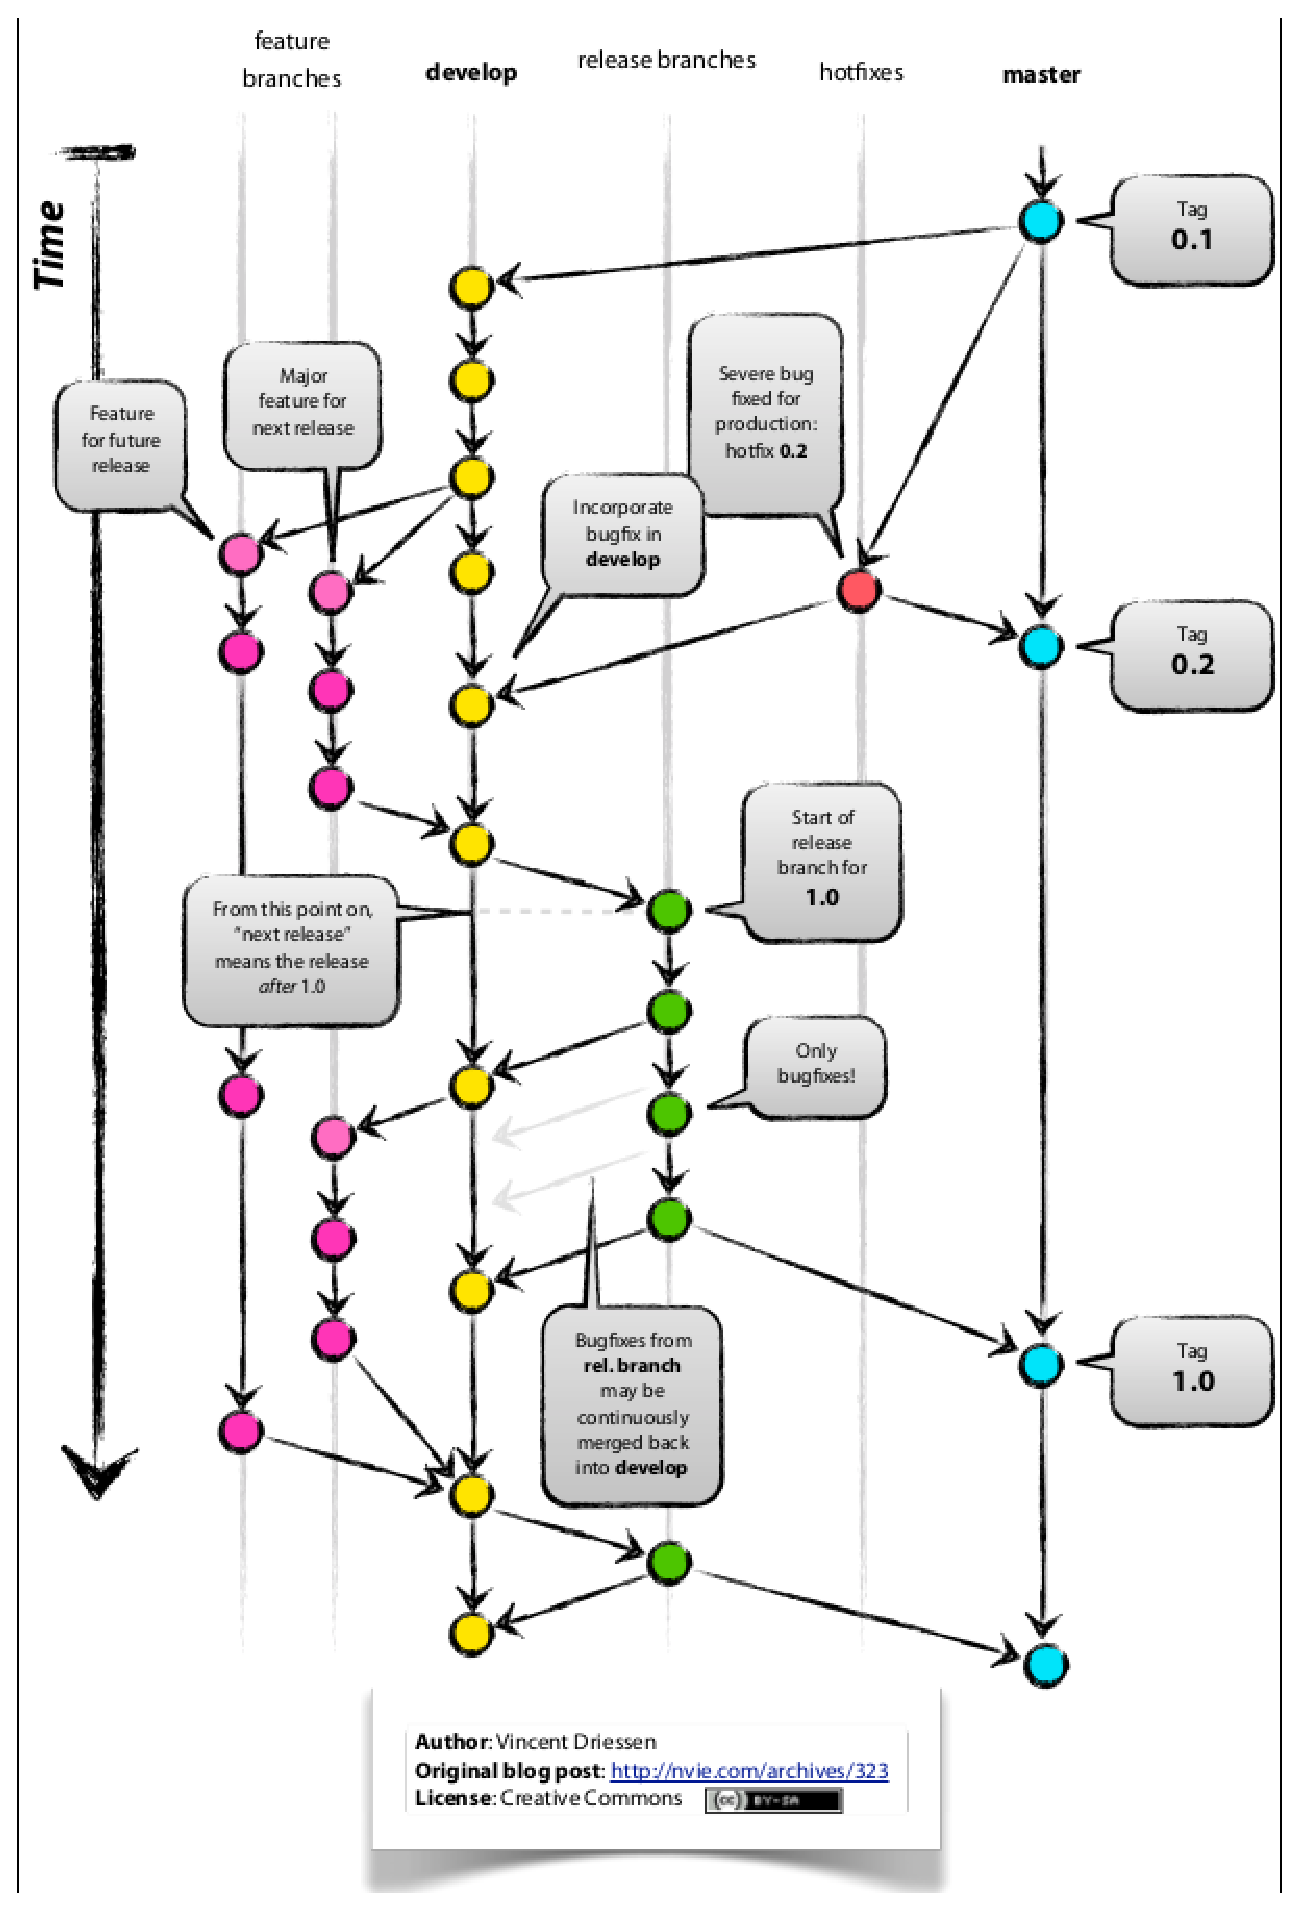
\includegraphics[width=0.95\columnwidth]{Git-branching-model.eps}
%\caption{Structure of a GIT repository}
%\end{figure}
Here is a short summary:
\paragraph{Main permanent branches}
The repository should have two permanent branches:
\begin{itemize}
\item The \textit{develop} branch, that contains commits as small as possible. This branch gives the detailed history of all the modification that have been realized on the repository. 
\item The \textit{master} branch, that contains released version only. They \textbf{must} work. The corresponding commits may be huge, since they correspond to squashes of commits that have been pushed in the develop branch.
\end{itemize}

\paragraph{Extra permanent branches}
Other permanent branches can be created, corresponding to important demonstration or papers.
Those repositories should be stored in the root of the git repository.

\paragraph{Temporary branches}
Next to those branches, other branches can be created for several reasons:
\begin{itemize}
\item Develop new features. At the end of the test process, the commits should be \textit{rebased} with the release branches.
\item Develop a hotfix. Once done, that are merged with both the master and the develop branch. 
%\item Develop a release. Once done, that are merged with both the master and the develop branch. 
\end{itemize}

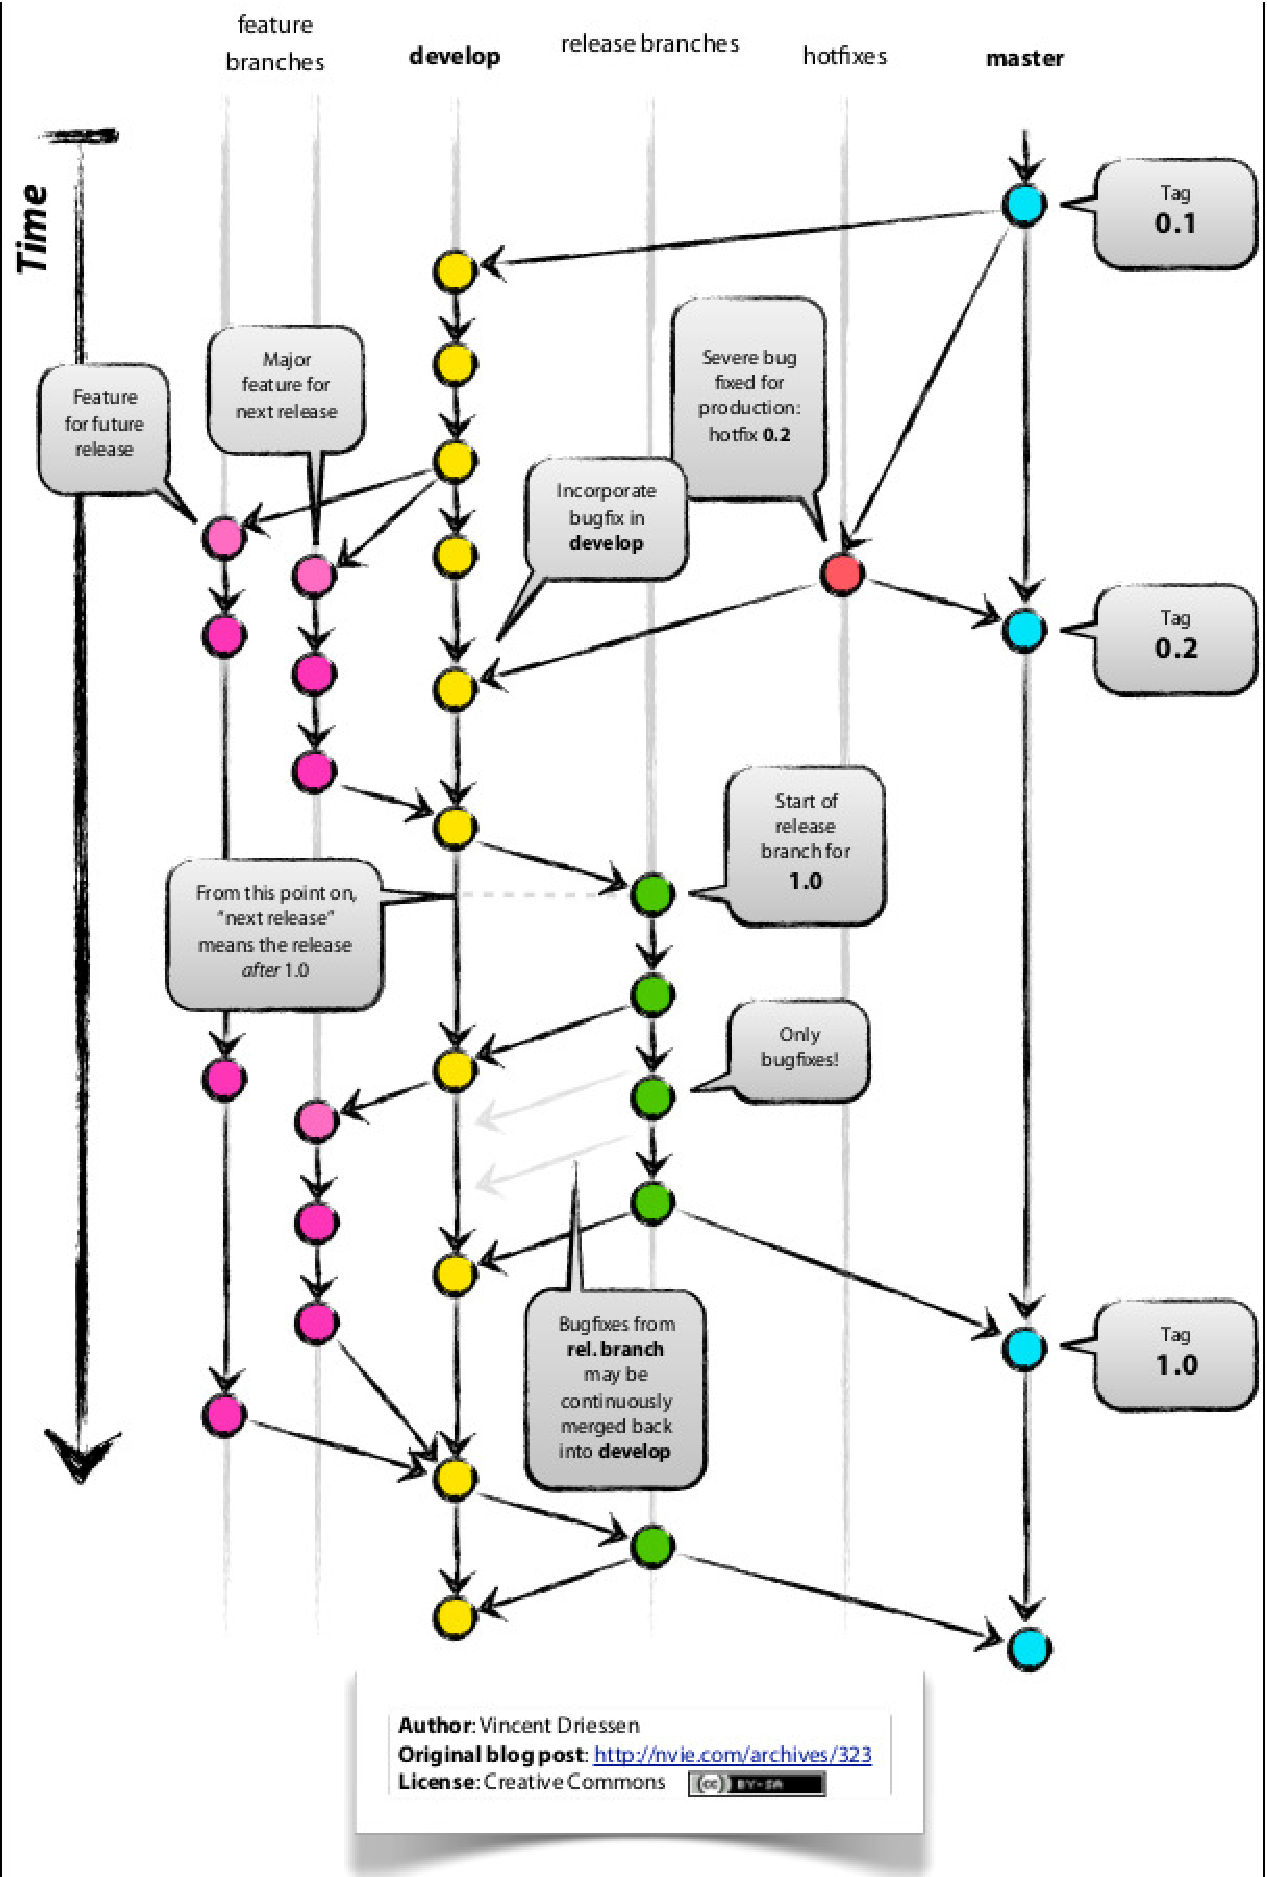
\includepdf[pages={1}]{img/Git-branching-model.pdf}

%\paragraph{Rebasing huge branches}
%\note{Robohow fellows: I'd like your opinion on the following issue:}
%The policies "every commit of the master can be computed" and "Use git --rebase" may conflict, especially 
%when the branch merged with the master branch is huge.
%Two solutions are possible:
%\begin{itemize}
%\item use the possibilities offered by git rebase to modify the commits (e.g. squash them).
%\item realize a merge with the master, so as to purposefully create a "circuit". 
%This offers the possibility to explore the commits realized in the branch (while ensuring that every commit in the master branch is functional).
%\end{itemize}


\section{Working in community}

\paragraph{Modifying an external package}
If you have write access to the remote repository, you can commit your modification, push them in a new remote branch (\begin{tt}git push origin patch/improvement\end{tt}), ask for verification from the main developers that will do/authorize the merge with the master branch. \\


If you do not have write access to the remote repository, commit the modification on your local repository and create the corresponding patches using the command 
\begin{tt}git format-patch reference\_commit -o out\_folder\end{tt}\\
e.g. 
\begin{tt}git format-patch origin/master -o patches\end{tt}

This command will convert all the commits from the reference\_commit to the last one into applicable commits,
and store them in the folder \textit{patches}

Thus, the main developers will be able to directly apply your patches using the command
\begin{tt}git apply patch\end{tt}\\

\textbf{Do NOT} do \begin{tt}git diff > patch.txt\end{tt}
This will create a file that is not directly usable, and the developers will have to recode your modifications.

\paragraph{Using others' packages}
Prefer working with tagged versions, that are more likely to be stable, and are better reference points.


\section{Forbidden practices}
Briefly, it is forbidden to modify a commit that has already been pushed. 
Such operations are likely to damage the remote repository and/or the repository of other users.
In particular, the following practices should be prohibited: 
\begin{itemize}
\item Forcing a push. Never use the command \begin{tt}{git push -f}\end{tt}
\item Changing a commit after pushing it. Once pushed, it is too late to do a \begin{tt}{git commit –amend}\end{tt}
\item Rebasing a branch that you pushed, or that you pulled from another person. 
Rebasing published branches can lead to duplicate commits in the shared repository.
\end{itemize}

The only exception to these rules is when a file that should not been distributed has been pushed (file containing a password, sensitive informations \ldots).
In this case, you can destroy the wrong commit by using \begin{tt}push -f\end{tt} and/or contacting the main person in charge of the code to explain what happened.

\section{Sources}

\paragraph{General guidelines}~\\
\small{\url{https://wiki.duraspace.org/display/FCREPO/Git+Guidelines+and+Best+Practices}}\\
\small{\url{http://goo.gl/H5OnA}}\\

\paragraph{Commit message shape}~\\
\small{\url{http://tbaggery.com/2008/04/19/a-note-about-git-commit-messages.html}}\\

\paragraph{About the merge and the rebase}~\\
\small{\url{http://darwinweb.net/articles/the-case-for-git-rebase}}\\
\small{\url{http://jeffkreeftmeijer.com/2010/the-magical-and-not-harmful-rebase}}\\
\small{\url{http://nvie.com/posts/a-successful-git-branching-model}}\\
%\end{document}